\documentclass[class=report, crop=false]{standalone}
\usepackage[subpreambles=true]{standalone}
\usepackage{import}
%%\usepackage{booktabs}
%\usepackage{tikz}

%\usepackage[utf8]{inputenc}
\usepackage[subpreambles=true]{standalone}
\usepackage{import}
\usepackage{pgfplots}
\pgfplotsset{compat=newest}
\usepgfplotslibrary{groupplots}
\usepgfplotslibrary{dateplot}
\usepackage{caption}
\usepackage{subcaption}
\usepackage{graphicx}
\usepackage{amsmath}
\usepackage{amssymb}
\usepackage[parfill]{parskip}
\usepackage{float}

% \usepackage{pgfplots}
% \usetikzlibrary{pgfplots.groupplots}
% \pgfplotsset{compat=1.9,height=0.3\textheight,legend cell align=left,tick scale binop=\times}
% \pgfplotsset{grid style={loosely dotted,color=darkgray!30!gray,line width=0.6pt},tick style={black,thin}}
% \pgfplotsset{every axis plot/.append style={line width=0.8pt}}
%
% \usepgfplotslibrary{external}
% % Für die Verwendung von 'external' müssen die folgenden Anpassungen in Abhängigkeit der
% % LaTeX Distribution durchgeführt werden:
%
% % fuer Texlive: pdflatex.exe -shell-escape -synctex=1 -interaction=nonstopmode %.tex
% \tikzexternalize[shell escape=-shell-escape]   % fuer TeXLive
%
% % fuer MikTeX:  pdflatex.exe -enable-write18 -synctex=1 -interaction=nonstopmode %.tex
% %\tikzexternalize[shell escape=-enable-write18] % fuer MikTex
%
%
%
% \tikzsetexternalprefix{graphics/pgfplots/} % Ordner muss ev. zuerst haendisch erstellt werden

\begin{document}

\section{Octagon}\label{sec:octagon}

We set up an experiment where we can observe drifts and test the accuracy of our system. We taped down 8 straight equidistant lines with 1.5 meter distance from the middle and marked the 1.5 meter mark on the tape. This way if we drive our robot from point to point, the path will be an octagonal shape where we can see drifts in accuracy over longer periods if we do multiple loops through the same path.

\begin{figure}[H]
    \centering
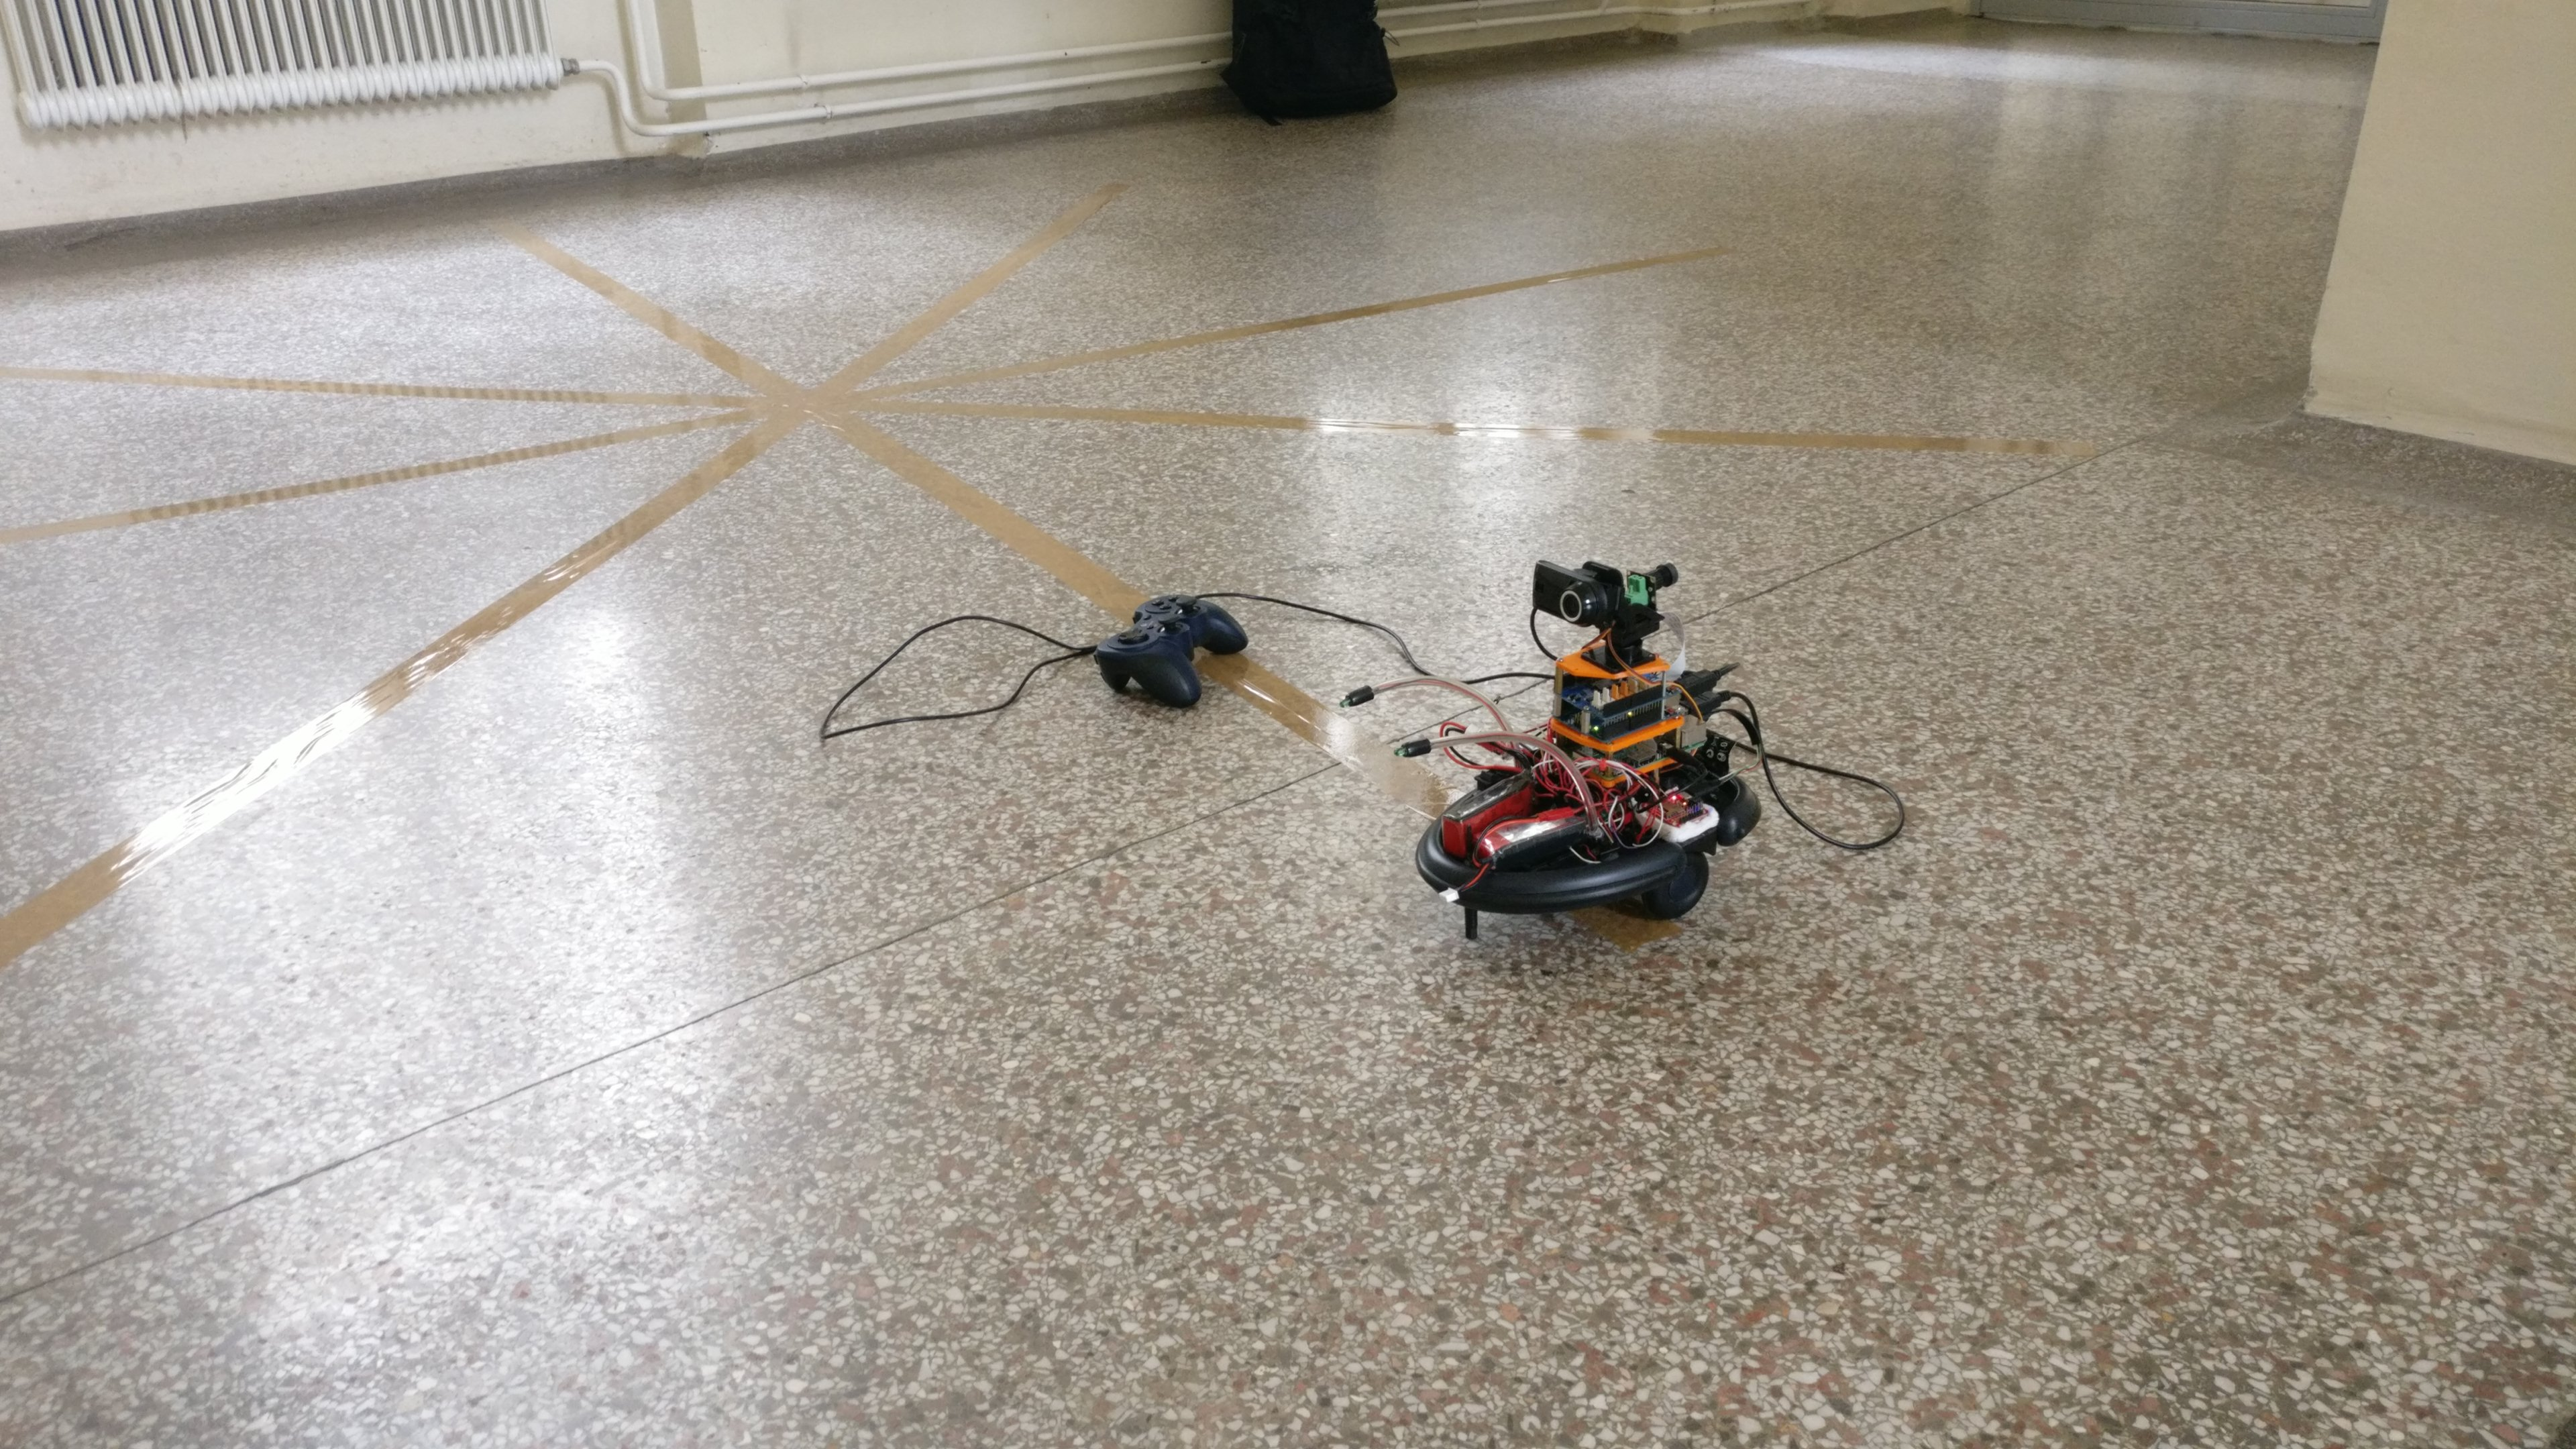
\includegraphics[width=10cm, height=5cm]{images/octagon.jpg}
\caption{Octagon experiment setup: 8x 3 meter long tape on the floor with their centers on top of each other in 45\si{\degree} spacing.}
\end{figure}\label{fig:octagonexp}

\begin{center}
\begin{figure}[H]
  \begin{tikzpicture}
   \begin{axis}[
     yticklabel style={
       /pgf/number format/fixed,
       /pgf/number format/precision=5
      },
     width=12cm,
     height=12cm,
     xmin=-2.5, xmax=2.5,
     ymin=-3.5, ymax=1.5,
     xlabel={x state [m]},
     ylabel={y state [m]},
     xtick distance= 0.5,
     ytick distance=0.5,
     legend pos=north west,
     grid=both,
     grid style={
       line width=.1pt,
       draw=gray!10},
     major grid style={
       line width=.2pt,
       draw=gray!50
      },
    ]
    \addplot+[color=red, mark=none,line width=1pt,mark size=1pt, dashed] table {plots/octagon0_x0x1.csv};
    \addlegendentry{KF}
    \addplot+[color=blue, mark=none,line width=1pt,mark size=1pt] table {plots/octagon1_x0x1.csv};
    \addlegendentry{KF(APN)}
    \filldraw [fill=black, draw=white, thick] (axis cs:0,0) circle [radius=4pt] node[anchor=north] {Start};
    \filldraw [fill=blue, draw=white, thick] (axis cs:3.900866408655341844e-01, 7.026190321121479343e-01) circle [radius=4pt] node[anchor=north] {End};
    \filldraw [fill=red, draw=white, thick] (axis cs:-1.281200888097691615e-01, 2.669405901909106538e-01) circle [radius=4pt] node[anchor=north] {End};
   \end{axis}
  \end{tikzpicture}
 \caption{Comparison of x-y trajectory estimates with the Kalman filter and Kalman filter with adaptive process noise after driving through the octagon multiple times. KF(APN) overshoots due to higher gyroscope reliance.}\label{fig:octagonxy}
\end{figure}
\end{center}

The robot wasn't driven perfectly due to difficulties in turning accurately, but we can observe drifts due to accumulating errors in the $\Psi$ state. This error gets bigger with KF(APN) due to higher reliance on the gyroscope.

A steady balance between model and measurement seems to yield better results with a well set $\varrho_{\eta\chi}$ ratio, similar to in Section \ref{sec:floor}.

\vspace{0.5cm}

\begin{center}
\begin{figure}[H]
  \begin{tikzpicture}
   \begin{axis}[
     yticklabel style={
       /pgf/number format/fixed,
       /pgf/number format/precision=5
      },
     width=12cm,
     height=12cm,
     xmin=-3.0, xmax=2.0,
     ymin=-3.5, ymax=1.5,
     xlabel={x state [m]},
     ylabel={y state [m]},
     xtick distance= 0.5,
     ytick distance=0.5,
     legend pos=north west,
     grid=both,
     grid style={
       line width=.1pt,
       draw=gray!10},
     major grid style={
       line width=.2pt,
       draw=gray!50
      },
    ]
    \addplot+[color=red, mark=none,line width=1pt,mark size=1pt, dashed] table {plots/octagon0_x0x1.csv};
    \filldraw [fill=red, draw=white, thick] (axis cs:-1.281200888097691615e-01, 2.669405901909106538e-01) circle [radius=4pt] node[anchor=north] {End};
    \addlegendentry{KF}
    \addplot+[color=blue, mark=none,line width=1pt,mark size=1pt] table {plots/octagon2_x0x1.csv};
    \filldraw [fill=blue, draw=white, thick] (axis cs:5.240493095723061101e-01, -1.681197626578265492e-01) circle [radius=4pt] node[anchor=north] {End};
    \addlegendentry{mistuned KF}
    \filldraw [fill=black, draw=white, thick] (axis cs:0,0) circle [radius=4pt] node[anchor=north] {Start};
   \end{axis}
  \end{tikzpicture}
 \caption{Effects of mistuning the $\varrho_{\eta\chi}$ parameter by 150\% on the x-y trajectory after driving through the octagon shape multiple times. It overshoots by around 0.5 meters.}\label{fig:octagonmistuned}
\end{figure}
\end{center}

\end{document}
